%% ==============================
\chapter{\iflanguage{ngerman}{Methoden}{Methods}}
\label{sec:methods}
%% ==============================

Nachdem beschlossen wurde, dass diese Arbeit sich an dem Clusteringverfahren aus dem Paper von Nguyen \cite{nguyen2012clustering} orientiert, werden in diesem Kapitel die verschiedenen verwendeten Methoden vorgestellt.

\subsection{Gradient}

Zuerst müssen die Gradienten aller Voxel berechnet werden. Dafür wurde Hong's Methode \cite{hong2003method} gewählt. Diese ist ein Approximation-basiertes Verfahren zur Berechnung von Gradienten eines Volumens unter der Betrachtung der lokalen 4x4x4 Nachbarschaft des Punktes.
\newline
Hierbei ist zu beachten, dass es nicht möglich ist, den Gradienten für einen Voxel direkt zu berechnen. Der Gradient drückt die Veränderung der Intensitätswerte im Raum aus, folglich kann er immer nur zwischen mehreren Punkten berechnet werden. Deshalb liegt er im Falle eines dreidimensionalen Volumens im Zentrum eins Würfels, der von 8 benachbarten Voxeln aufgespannt wird.
\newline
In \autoref{fig:nachbarschaft} ist zu erkennen, wie der Gradient im Zentrum der acht Voxel liegt. Des Weiteren ist die 4x4x4 Nachbarschaft in Form der durchnummerierten Punkte zu sehen.
\newline

\begin{figure}[!h] 
\centering 
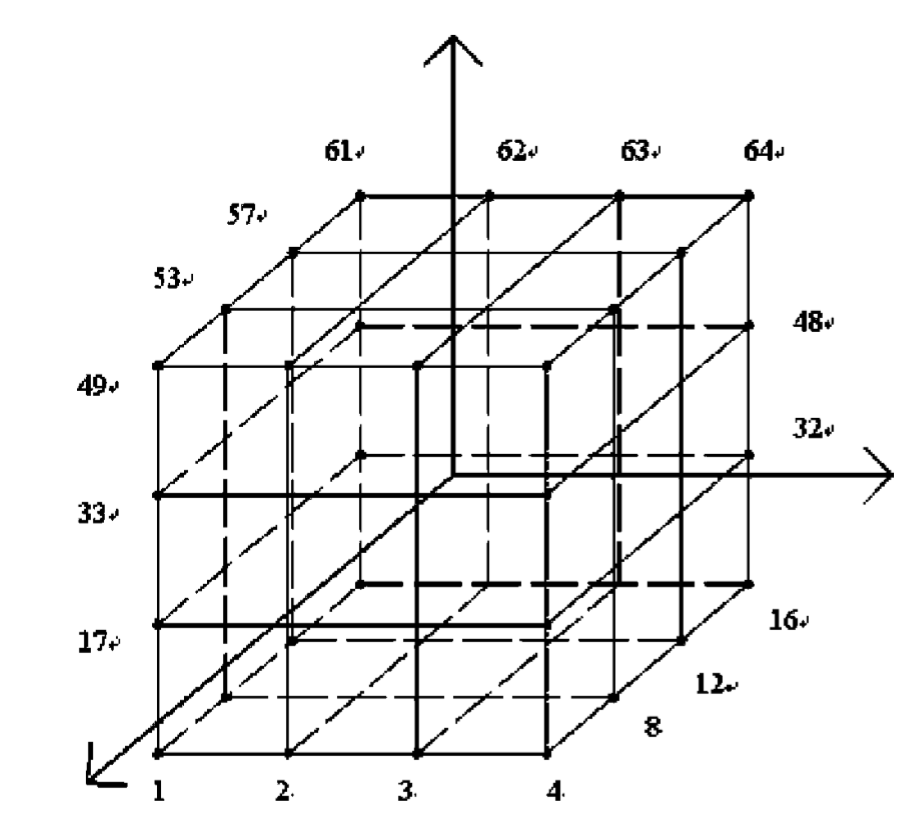
\includegraphics[width=0.75\textwidth]{Logos/VoxelEdges.PNG}
\caption{Darstellung der lokalen 4x4x4 Nachbarschaft  \\ Entnommen aus \protect\cite{hong2003method}} 
\label{fig:nachbarschaft} 
\end{figure}


Ein Gradient ist ein dreidimensionaler Vektor, der in die Richtung der größten Änderung der Intensitätswerte im Volumen zeigt. Gäbe es eine Funktion, die die Intensitätswerte des Volumens beschreibt, wären der Gradient folglich die Ableitung dieser Funktion. Deshalb muss für die Berechnung eines Gradienten zunächst eine Intensitätsfunktion für die lokale 4x4x4 Nachbarschaft aufgestellt werden. Im Paper wird dies mit der Formel:
\begin{equation}
	f(x,y,z) = Ax^{2}+By^{2}+Cz^{2}+2Fyz+2Gzx+2Hxy+2Ix+2Jy+2Kz+D
\end{equation}
approximiert, da es nicht möglich ist eine solche Funktion zu bestimmen. Um den Gradienten zu erhalten muss, wie gesagt, diese Funktion abgeleitet werden. Zur Berechnung des Gradientenvektor $n$ ergibt sich dadurch die Formel:


\begin{equation}
	n =2\begin{bmatrix}
           Ax + Gz + Hy + I \\
           Hx + By + Fz + J \\
           Gx + Fy + Cz + K
         \end{bmatrix} 
\end{equation}


Um zu messen, wie gut die Approximation die Intensitätswerte beschreibt, wird im Paper die \textit{error distance} vorgestellt, die die Entfernung zwischen einem berechneten Datenpunkt und seinem korrespondierenden Punkt in den tatsächlichen Daten beschreibt. Die Funktion $E(A,B,C,D,F,G,H,I,J,K)$ beschreibt die Summe der \textit{error distance} aller Punkte.


\begin{equation}
  E(A,B,C,D,F,G,H,I,J,K) = \sum\limits_{k=1}^{64}  w_{k}(Ax^{2}+By^{2}+Cz^{2}+2Fyz+2Gzx+2Hxy+2Ix+2Jy+2Kz+D - f_{k})^2
\end{equation}

Dabei ist $w_{k} = \frac{1}{d_{k}}$, $d_{k} =(x_{k}^2y_{k}^2z_{k}^2)^{1/2}$  die Distanz des k-ten Punktes zum Ursprung des Koordinatensystems, wie es in \autoref{fig:nachbarschaft} zu sehen ist und $f_{k}$ der Intensitätswert des k-ten Punktes. Die Parameter $A,B,C,E,F,G,H,I,J,K$  der Funktion müssen so gewählt werden, dass die Summe $E$ minimal wird, damit die approximierte Intensitätsfunktion das Volumen möglichst genau beschreibt. Die Parameter können deshalb mithilfe der Methode der kleinsten Quadrate bestimmt werden. Dies ist ein mathematisches Verfahren, das zu mehreren Punkten, eine Funktion bestimmt. Die Funktion beschreibt eine Kurve, bei der die Summe der Abweichung aller Punkte zur Kurve minimal ist. Mithilfe dessen können durch mehrere Umformungsschritte die Parameter berechnet werden. Anschließend kann der Gradient $[X, Y, Z]$ des Punktes $[x, y, z]$ mit folgender Formel, die sich aus der Ableitung des Intensitätsfunktion ergibt, kalkuliert werden:


\begin{align}
\begin{bmatrix}
           X \\
           Y \\
           Z
         \end{bmatrix}    
 	= \begin{bmatrix}
           2A & 2H & 2G \\
           2H & 2B & 2F \\
           2G & 2F & 2C
         \end{bmatrix}
         \begin{bmatrix}
           x \\
           y \\
           z
         \end{bmatrix}
	+\begin{bmatrix}
           2I \\
           2J \\
           2K
         \end{bmatrix}
  \end{align}



\subsection{LH-Werte}

Als nächster Schritt folgt die Berechnung der Low- und High-Werte. Diese beschreiben die Grenzen zwischen zwei verschiedenen Materialien. Liegt ein Voxel innerhalb eines Materials, so sind seine LH-Werte gleich. Liegt ein Punkt jedoch an der Grenze zweier Strukturen, so beschreibt der Low-Wert den Intensitätswert des Materials mit dem niedrigeren Intensitätswert und der High-Wert, das Material mit dem höheren Intensitätswert. Die LH-Werte eines Voxels werden berechnet, indem in die Richtung des Gradienten integriert wird. Hierfür wurde Heun's Methode, eine modifizierte Euler Methode, verwendet. Die für die Integration benutzte Formel lautet:
\begin{equation}
	u_{i+1} = u_{i} + \frac{1}{2}d(\triangledown f (u_{i}) + \triangledown f(u_{i}+d \triangledown f(u_{i}))) 
\end{equation}
Hierbei sind $u_{i}$ und $u_{i+1}$ die Positionen des aktuellen, beziehungsweise des nächsten Voxels. $\triangledown f(x)$ beschreibt den normalisierten Gradienten bei der Berechnung der High-Werte und den normalisierten inversen Gradiente bei der Berechnung der Low-Werte des Punktes $x$ . $d$ steht für die Schrittweite, die in dieser Arbeit auf einen Voxel festgelegt wurde.
\newline
Die Integration stoppt, wenn eine lokale Extremstelle oder ein Wendepunkt erreicht wird. Diese sind daran zu erkennen, dass die Längen der Gradienten an diesen Stellen null sind.
\newline
Wird ein solcher Punkt erreicht, wird der Intensitätswert des aktuell besuchten Voxels als Ergebnis für den Low- beziehungsweise High-Wert des Startvoxel gespeichert.
\newline
Anschließend wird ein LH-Histogramm mit allen berechneten LH-Wertpaaren erstellt. Hierbei sind auf der x-Achse die Low-Werte und auf der y-Achse die High-Werte angesiedelt. Die Werte der Achsen reichen von null bis zum jeweiligen Maximum der Low- beziehungsweise High-Werte.



\subsection{LH-Clustering}

Als nächstes, wird der erste Clusteringschritt durchgeführt. Dieser findet über dem LH-Raum, genauer gesagt auf dem eben berechneten LH-Histogramm statt. Dafür wird \textit{Meanshiftclustering} verwendet.
\newline
Vor dem Berechnen der Cluster muss zunächst eine Bandweite sowie ein Thresholdwert bestimmt werden, welche die Sensitivität des Clusterings angeben. Die von Nguyen \cite{nguyen2012clustering} verwendete Bandweite liegt bei 7\% bis 9\% des maximalen LH-Wertes und der Threshold bei 0,01. Anschließend kann die Kalkulation der Cluster beginnen.
\newline
Für einen beliebigen Punkt, werden alle Punkte die innerhalb des Radius der Bandbreite liegen gespeichert. Diese Punkte bilden den gefundenen Cluster. Von diesem Cluster wird der Mittelpunkt berechnet, indem jeweils die L- und die H-Werte aller Punkte des Clusters aufaddiert und durch die Anzahl der Punkte geteilt wird. Um den neuen Mittelpunkt werden wieder alle Punkte, die innerhalb des Radius liegen und noch nicht zum Cluster gehören, hinzugefügt und anschließend erneut ein neuer Mittelpunkt berechnet. Dies geschieht solange, bis die Distanz des neu kalkulierte Mittelpunkt zum alten kleiner als der Thresholdwert multipliziert mit der Bandweite ist. 
\newline
Nachdem diese Prozedur für jeden Punkt im Histogramm ausgeführt wurde, existieren viele Cluster, die oftmals aus vielen gleichen Punkten bestehen. Um dies zu unterbinden werden in einem weiteren Schritt alle Cluster die sehr nah beieinander liegen verschmolzen. Dies betrifft jene Cluster, deren Mittelpunkte eine Distanz kleiner als die Hälfte der Bandweite zueinander haben.



\subsection{Räumliches-Clustering}

Als nächster Schritt, wird erneut auf jedem eben entstandenen Cluster \textit{Meanshiftclustering} angewendet. Dabei wird auf jedem Cluster einzeln und unabhängig von den anderen Clustern geclustert. Außerdem werden diesmal die räumlichen Informationen der Punkte in Betracht gezogen. Hierzu müssen zunächst erneut die beiden Parameter Bandweite und Threshold definiert werden.
\newline
Anschließend läuft das Clustering wie zuvor im LH-Raum ab, mit dem Unterschied, dass statt im zweidimensionalem Raum mit einem zweidimensionalem Kreis im dreidimensionalem Raum des Volumens mit einer dreidimensionalen Kugel nach Voxeln gesucht wird.
\newline
Des Weiteren findet am Ende der Berechnung der Cluster keine Verschmelzung statt, da dies den Sinn der beiden verschiedenen Clusteringschritte zerstören würde. In den finalen Cluster haben alle Punkte jeweils ähnliche LH-Werte und liegen im Volumen nah beieinander.
\newline
Würden diese Cluster anhand ihrer räumlichen Informationen verschmolzen werden, hätten die Punkte keine ähnlichen LH-Werte mehr und der erste Clusteringschritt wäre umsonst gewesen.



\subsection{Hierarchisches-Clustering}
 
Im optionalen letzten Clusteringschritt, werden die berechneten Cluster hierarchisch miteinander verschmolzen. Dafür wird zunächst der paarweise Abstand zwischen allen Clustern berechnet. Der Abstand wird wie bei Sereda \cite{sereda2006automating} anhand der Anzahl der direkten Nachbarschaften der Voxel beider Cluster bestimmt. Anschließend werden immer die beiden Cluster die sich am nächsten sind zu einem verschmolzen. Dieser Vorgang wiederholt sich so lange, bis nur noch ein Cluster existiert. Im Anschluss wird das Verfahren Schritt für Schritt rückgängig gemacht, bis eine vom Benutzer angegebene Anzahl an Clustern erreicht wird.
\newline
Der vorgestellte dritte hierarchische Clusteringsschritt wurde in dieser Arbeit nicht angewendet. Dies wurde aus dem Grund entschieden, dass das Verschmelzen von Clustern abhängig von räumlicher Nähe für die Aufgabe das Ventrikelsystem hervorzuheben nicht zielführend ist. Wird das System als ein oder mehrere Cluster erkannt, liegen diese mitten im Gehirn neben sehr vielen anderen Clustern und würden vermutlich meistens mit anderen umliegenden Strukturen verschmolzen werden.

